% Chapter Template

\chapter{Case Study} % Main chapter title

\label{chapter-case_study} % Change X to a consecutive number; for referencing this chapter elsewhere, use \ref{ChapterX}

\lhead{Chapter . \emph{Case Study}} % Change X to a consecutive number; this is for the header on each page - perhaps a shortened title



\section{Human-Aware Robot Guide}
\subsection{Introduction}
%Introduction
%One interest of the recent research is for social robots that interact with users to help them accomplish a range of tasks. 
One interesting problem in human-robot interaction is developing robots able to guide humans, by offering a tour of attractions in an area or simply by helping humans to reach a destination.
%There is a big interest today in social robots that interact with users to help them accomplish a range of tasks. 
%Some deployed in domestic environments and others in public spaces, like amusement parks or museums. 

%%Characteristics
A generic mobile robot platform should possess a vast set of skills, which includes advanced perception, motion planning, and task planning. These skills are not enough for a robot guide, which is deployed in highly dynamic human environments, and need to be complemented with human-aware behaviors.

%Examples
Different robot guides have been studied and developed, starting with pioneers like Rhino and Minerva \cite{thrun2000probabilistic}. After these first experiments, several researchers have tried to focus on the social aspects of the problem, which are especially important if the robot needs to offer information. Studies like \cite{yousuf2012development,evers2014development} focus on how the robot should address humans, concentrating on spatial relationships and on how the robot can convey information. Few systems have actually been deployed for long period of time in human environments. Rackhman \cite{clodic2006rackham}, a museum guide with human-aware behaviors, is an example of such system, and has been deployed in a science museum for several months. 
%
%The authors collected information about the interactions between Rackhman and visitors of the museum to improve their knowledge about human-robot interaction.
%\cite{bueno2011autonomous} integrates a robot museum guide in a smart environment, using virtual avatars with human-aware interfaces associated to exhibitions in order to convey information to the users.
%
Robotic systems must be able to reason on sensor data in order to provide information to the decision layers. In \cite{Milliez2014}, we presented our framework \emph{SPARK}, which is able to maintain a topological description of the world state and  to reason on humans' mental states, in order to improve the robot's social behavior. For guiding situations, \cite{Jensen2005} presents an assessment of human-robot interaction during an exhibition, where perceptual and task related data are used to compute an internal state according to the scenario. With these information, the robot can compute a new emotional state and interact accordingly with users.
Recently there has been emphasis on robot navigation algorithms that explicitly reason about human beings in the environment differently from other static or dynamic obstacles. Starting from \textit{Proxemics}, researchers have investigated explicit social signals based on human-posture and affordance of the environment to improve legibility of robot motion. For detailed discussion on human-aware navigation algorithms we refer the readers to \cite{kruse2013human,rios-ijsr-2014}. Human-aware navigation in a museum situation was studied in \cite{samejima2015building}, where the authors build environmental maps, which include information learnt from human trajectories and postures, in order to plan safe paths that don't disturb humans present in the area. 

%
Or \cite{rashed2015toward}, which is related to a museum scenario. 

Humans tend to naturally form groups, which can be classified in different types, based on their size, on their level of cohesion, on their duration, and other factors \cite{forsyth2009group}. %Studying and representing group formations is important to build human-aware robots.
Studying group formations is a complex problem, since the robot must be able to detect humans, which can be occluded in populated environments, and to model their social interactions, which can be ambiguous. One of the most powerful and expressive social cues is distance, used in different works to track social relationship, like \cite{luber2013multi}. 
%
%Our Model

We believe that most robot guide systems are focusing on the social aspects of the problem, and on human-aware navigation, without fully considering the fundamental aspects of joint actions. Guiding is a collaborative task, where the robot doesn't need only to reach a destination, but also to ensure that its followers reach it, while providing a socially acceptable experience to them. In order to achieve this goal, the robot needs to constantly monitor its users, to adapt to their behaviors and to be ready to proactively help them.

In this paper, we present a robot guide which is able to lead a group of people to a destination. More particularly, the originality of our approach is that the robot is able to show both an adaptive and a proactive behavior. The robot will try, while guiding, to select a speed that pleases its users, when adapting, or to propose a new speed, using environmental and task related stimulus. Finally, our system will proactively try to engage members of the group if it detects they need assistance. 

We implement these ideas using a Situation Assessment component, which gathers data from different sources and provides symbolic information, a Supervision System, that controls the other modules, and a planning framework based on hierarchical MOMPDs (Mixed Observability Markov Decision Processes). Finally, a human-aware Motion Planning component allows the robot to navigate populated environments.
\vspace{-10pt}

\subsection{Environment-Based Intention Recognition}

To be relevant, reasoning on humans should be linked to the environment. The system is able to create activity areas in the environment and link them to different kind of computations. An activity area is a polygonal or circular area, which can be fixed or linked and updated with an entity's (object, human or robot) position. For now, we studied and experimented different activity areas: a) Information Screen Area, linked to information screens present in the environment; b) Touristic Point Area, linked to interesting attractions in the environment.
Using these areas, the system can detect human activities (e.g. human is looking at an information screen, human is looking at an attraction).


\subsection{Task and Motion Planning Problems}
A robot-guide will have to navigate big environment, often too big to perform efficiently motion planning, to reach its destination. A solution to this problem is reducing the size of the area where the motion planner will compute its paths, and splitting the navigation problem in a series of sub goals. The problem, with this approach,  is choosing the correct list of sub-goals  in order to reach the final position.  To deal with this issue we implemented an A* based task planner, which will choose a high-level path to be followed by the robot from a semantic map. This map is a hand-crafted graph. composed by different nodes, representing parts of the environemts (corridor, elevator entrance, gates area). Each node will be linked to a point in the real world. At the end of planning the robot will procuce a list of coordinates usable by the motion planning layer. 

A first possibility to manage a plan is simply travelling to each point in the map, sending a goal to the motion planner for the next point. The problem with this approach is that the path followed by the robot might be very inefficient, as shown in the figure %put figure.
To reduce the size of the planning area we used a rolling window approach, where the motion planner will plan on a grid map centered on the robot, which will move with it. In this way, the robot will send the next goal in the calculated plan as soon as its present in the rolling window. It's very important, with this approach to carefully select compute the nodes in the semantic maps so that the rolling window will contain at least two semantic nodes. If not, the motion planner will have to plan for a goal outside its grid map, which will generate an error.


\subsection{Collaborative Planner to Guide a Group}
We use a hierarchical framework \cite{pineau2001hierarchical}, where the system model is split into a main MOMDP module and several MOMDP sub-models, each one related to a different action. The models are solved separately, leading to the computation of different, simpler, policy functions. At run-time, the system interacts with the main module, providing values for the set of observations and for the observed variables, and receiving an action as result. Based on this action, the system will contact a different sub-model, receiving the final action to execute. Using hierarchical MOMDPs we can represent a set of models, with a greatly reduced complexity, and easily expand it if we want to implement new actions or to add more complex behaviors.  The architecture of our system is shown in Figure \ref{architecture} A).


\begin{figure}[h!]
 \vspace{-20pt}
\caption{A) System Architecture: our system is composed by four main modules. Situation Assessment reasons on perceptual data, providing symbolic information to the Supervision System. The Supervision System controls the other modules, updating the Collaborative Planners, which compute the next action to perform, and sending goals to the Motion Planning. Blue arrow represent data links between modules, while red arrows represent conceptual links that show the hierarchy of the MOMDP. B) The robot guiding a user.}
\label{architecture}

  \centering
\includegraphics[trim={30cm 5.2cm 0 2cm},clip,scale=0.38]{img/architecture_conceptual_2.pdf}
\vspace{-20pt}
\end{figure}

\vspace{-5pt}
\subsubsection{Guiding the Group}
The main problem of the robot is choosing if it should still guide the group, suspend temporarily the task, or abandon it. The Guide Planner is the main MOMDP of our architecture and will make this decision, based on two main variables: the status of advancement of the task (\textit{not\_completed}, \textit{completed}), and the quality of commitment of the group (\textit{not\_engaged}, \textit{engaged}, \textit{not\_interested}). The quality of commitment of the group is an hidden variable, estimated using  Situation Assessment, based on the distance of the group toward the robot, its variation, if the members of the group are oriented toward the robot, and if they are moving or still. The robot will abandon the task when it evaluates that the group of followers is empty, as explained in Section \ref{situationAssessment}.

\vspace{-5pt}
\subsubsection{Adapting the Robot's Speed}
We believe that to be socially acceptable, the robot should adapt its speed to the group. By setting its own pace at the start of the scenario the robot  would risk of being too slow, annoying the users, or too fast, which would lead the robot to constantly stop to wait for the group, producing an awkward behavior.

The robot defines a desired range of distance $r$ from the group. The distance of the  members of the group from $r$ will influence its actions. 1) If there is a member of the group farther than $r$ the robot will \textit{decelerate}. The main goal of a guide robot should still be guiding all of the group, and so the robot will give priority to people that would like a slower speed. 2) If 1) is false, and the majority of the group is closer to the robot than $r$, the robot will $accelerate$. 3) If 1) and 2) are false, the robot will continue at its pace.

% \begin{enumerate}
% \item if there is a member of the group farther than $r$ the robot will \textit{decelerate}. The main goal of a guide robot should still be guiding all of the group, and so the robot will give priority to people that would like a slower speed.
% \item if 1) is false, and the majority of the group is closer to the robot than $r$, the robot will $accelerate$.
% \item if 1) and 2) are false, the robot will continue at its pace.
% \end{enumerate}



%The robot defines a desired range of distance from the group during the task. When the majority of the group is closer than this range, the robot will estimate that the group wants to \textit{accelerate}.
%The main goal of a guide robot should still be guiding all of the group, and so the robot will give priority to people that would like a slower speed, estimated by computing that their distance from the robot is higher than the selected range, which will prompt the robot to \textit{decelerate}. 
In this paper, $r$ was a predefined vector of numbers, but its values could be learnt and adapted to the users during the task, since different people could prefer following the robot at different distances and positions.
The robot should also not constantly change speed, in order to give time to users to adapt to its new chosen speed, and so we defined a temporal threshold in which we don't allow the robot to repeat an \textit{accelerate} or \textit{decelerate} action.

In this scenario we also studied the idea that the robot can try to influence the speed of the group. We studied two situations in which this idea can be useful. A) There is a time limit to reach the destination. In this case the robot must balance the desire to satisfy the group with the task urgency. Different situations will require different policies. For example, in an airport scenario, the robot could prioritize arriving on time, warning users if their speed would render the goal not achievable, while in other situations the robot could try to arrive in time but still avoid to adopt speeds that are uncomfortable for the group. B) The rules of the current environment limit the robot's speed. In this case the robot will avoid accelerating over a set speed even if it detects that its current velocity is considered too slow for the group. For example, the robot could be navigating in a construction zone.
% \begin{itemize}
%    	\item There is a time limit to reach the destination. In this case the robot must balance the desire to satisfy the group with the task urgency. Different situations will require different policies. For example, in an airport scenario, the robot could prioritize arriving on time, warning users if their speed would render the goal not achievable, while in other situations the robot could try to arrive in time but still avoid to adopt speeds that are uncomfortable for the group.
%    	\item The rules of the current environment limit the robot's speed. In this case the robot will avoid accelerating over a set speed even if it detects that its current velocity is considered too slow for the group. For example, the robot could be navigating in a construction zone.
%     \end{itemize}

This reasoning is done in the Speed Adaptation MOMDP module, which will be interpreted when the Guide Model chooses to keep guiding the group.

\vspace{-5pt}
\subsubsection{Suspending the task}
In some situation, the robot needs to suspend the task, because the group has stopped following it. In this case, the robot should estimate if this suspension of the collaborative scenario is temporary or permanent, and in the latter case abandon the task. We estimate this information using the Suspend Model and the activity areas from Situation Assessment. We link activity areas to the maximum time we expect that the group will be involved in the linked activity, and with a set of proactive actions that the robot can choose to execute.

In this paper, we investigated a single possible proactive behavior: giving information. In this case, if we detect that one or more  members
of the group has stopped following because it is looking at a touristic sight, or at an information screen, the robot can try to engage him and offer related information. At the moment, we just propose a simple routine-based framework for this behavior, and plan to further study it in the future. We believe that the solution of this problem could be rich, and that the robot should estimate the reaction of the group during the execution of its proactive behavior, in order to be able to interrupt if the group doesn't want to be helped or to resume the original task if they are satisfied by the robot's actions.

We don't want the robot to be stuck for a long time  waiting for the group. If there is a small amount of time to reach the destination, or the group is engaged in the activity for a longer period of time than the one predicted, or the robot can't estimate the reason why the group stopped following, the Suspend Model can issue a warning action, and eventually abandon the task if the group doesn't start following it again.

%\subsection{Robot's reactiveness}
%When robots interact with humans in complex situations there is the risk that it will be too reactive to stimulus from the environment. To be socially acceptable, the level of reactivity of the robot needs to be controlled. As an example, we want to avoid that the robot continuously accelerates and decelerates, or stops and restarts moving, in order to adapt to the group's behavior. We investigated this problem both at the Situation Assesment level, using temporal reasoning, and the Planning Level, testing different time rates in order to interrogate the Collaborative Planners.

\vspace{-5pt}

\subsection{Motion Planning Notes}

A guiding robot need to plan safe and socially acceptable motion. This requires continual integration of high-level social constraints with the low-level constraints of the robot vehicle.

We use the architecture proposed by the well-established \verb!move_base! package of \verb!ROS! middle-ware \cite{movebase,ros} for navigation, replacing the global planner, i.e. a cost-grid base path planning module, as suggested in \cite{sisbotTRO2007}. This module adds proxemics based costs in the grid-map around the detected humans that are static in the environment. The local planner, i.e. the module responsible for generating motor commands, is a \textit{ContextCost} based algorithm suggested in \cite{kruse12crossing}. This module continuously calculates the \textit{compatibility} of the robot path by predicting and avoiding future collisions with moving persons and simultaneously keeping the robot as close as possible on the planned global path.

It should be noted that in our guiding experiments, the humans are mostly moving behind the robot and therefore the situation remains compatible for the local planner most of the time. During compatible situations the robot simply follows the way-points on the planned global path. The nominal velocity of the robot is set by the supervision system to achieve the desired behavior of slowing-down or speeding-up, as required by the situation. 

\vspace{-10pt}
\section{Laboratory Experiments and Analysis}
We performed a first set of experiments with a single user following a robot on a predefined path, in order to test the behaviors of the robot. After that, we tested the system by having a group of three users follow the robot. In this section, we show the results of our experiments on single user data, since they show in a clearer way the behavior of the system. We plan to perform, and present, user studies in the near future in order to analyze how groups of users react to the robot's behavior. Data from these experiments are shown in Table \ref{table:experiment results} \footnote{Videos from our experiments can be seen at http://homepages.laas.fr/mfiore/
icsr2015.html}. We start by showing speed adaptation tests:
\begin{itemize}
\item adapting slow and fast: in these two tests (Figure \ref{Fig:experiments}) we used our system to guide respectively a user that would like to move at a slow pace, and a user that would like to move at a fast speed.
\item no adaptation: in this experiments the robot won't adapt to the speed of the user, setting its own pace and stopping if it is too far.
\end{itemize}

Looking at the data we can see that our system shows lower values for the variance of speed and distance, which means that after a certain time it's able to find a condition of equilibrium with the human followers. The 'no adaptation' system shows a significantly higher variance for both values, since the robot stopped several times to wait for a user. We will now show some tests regarding the proactive behaviors of the robot:

\begin{itemize}
\item proactive slow and fast: during the task, the robot proactively chooses to change pace, in the first case by slowing down and in the second by accelerating. In our tests the user adapted after some seconds to the robot's pace, but this behaviors should be studied in-depth in user studies.
\item suspend with screen and with no reason: in these tests we asked a user to stop during the task. In the first case the user stopped near an information screen. After detecting this event, the robot approached the user to offer information, which lead to the resumption of the task. In the second case the user stopped at a different point of the path. The robot wasn't able to detect the reason for the suspension of the task and so simply   issued a warning to the user and abandoned the task after some seconds.
\end{itemize}


\begin{figure}[h!]
\caption{Experiments: a) Adapting robot speed to a slow user. The first figure shows the speed of the user ($tf\_to\_velocity/person\_1/linear/x$) and of the robot ($tf\_to\_velocity/robot/linear/x$), and the second their distance. The robot starts slowing down at $t=60$, when the distance from the user is growing, until it finds an equilibrium with the user's speed. Notice that there is a turn in the path, at $T=50$, that causes the robot and the user to slow down. Distances are expressed in meters, velocities in meters for seconds.
b) Adapting robot speed to a fast user. As before, the figures show the robot and user's speed and their distance. The robot starts accelerating at $t=15$  when the distance from the user becomes small.}
\label{Fig:experiments}

  \centering
 \includegraphics[trim={30cm 10cm 27cm 1cm},clip,scale=0.45]{img/architecture_conceptual_3.pdf}

\end{figure}

% \begin{figure}
% \centering
% \begin{minipage}{0.45\textwidth}
% \centering
% %\begin{table}
%  %\vspace{-20pt}
% %\caption{Experiment results: $d$ is the distance between the robot and the user; $s_r$ is the robot's speed, $s_h$ is the human's speed, $\mu$ is the average and $\Delta$ is the variation of the quantity.}
% %\centering
% \begin{tabular}{ | c | c | c | c | c | }

% \hline
%   test name     & $\mu$ $d$ & $\mu$ $s_r-s_h$ & $\Delta$ $d$ & $\Delta$ $s_r-s_h$ \\
% \hline
% adapting slow & 2.82 & -0.03 & 0.64 & 0.02 \\
%   \hline
%   adapting fast & 1.38 & 0.00 & 0.29 & 0.01 \\
%   \hline
%   no adaptation & 3.08 & -0.09 & 1.04 & 0.07 \\
% \hline
% proactive slow & 1.45 & -0.06 & 0.04 & 0.10 \\
% \hline
% proactive fast & 2.66 & -0.11 & 0.63 & 0.01 \\
% \hline
% \end{tabular}
% %\label{table:experiment results}
% % \vspace{-20pt}
% %\end{table}
% %\caption{first figure}
% \end{minipage}\hfill
% \begin{minipage}{0.45\textwidth}
% \centering
% 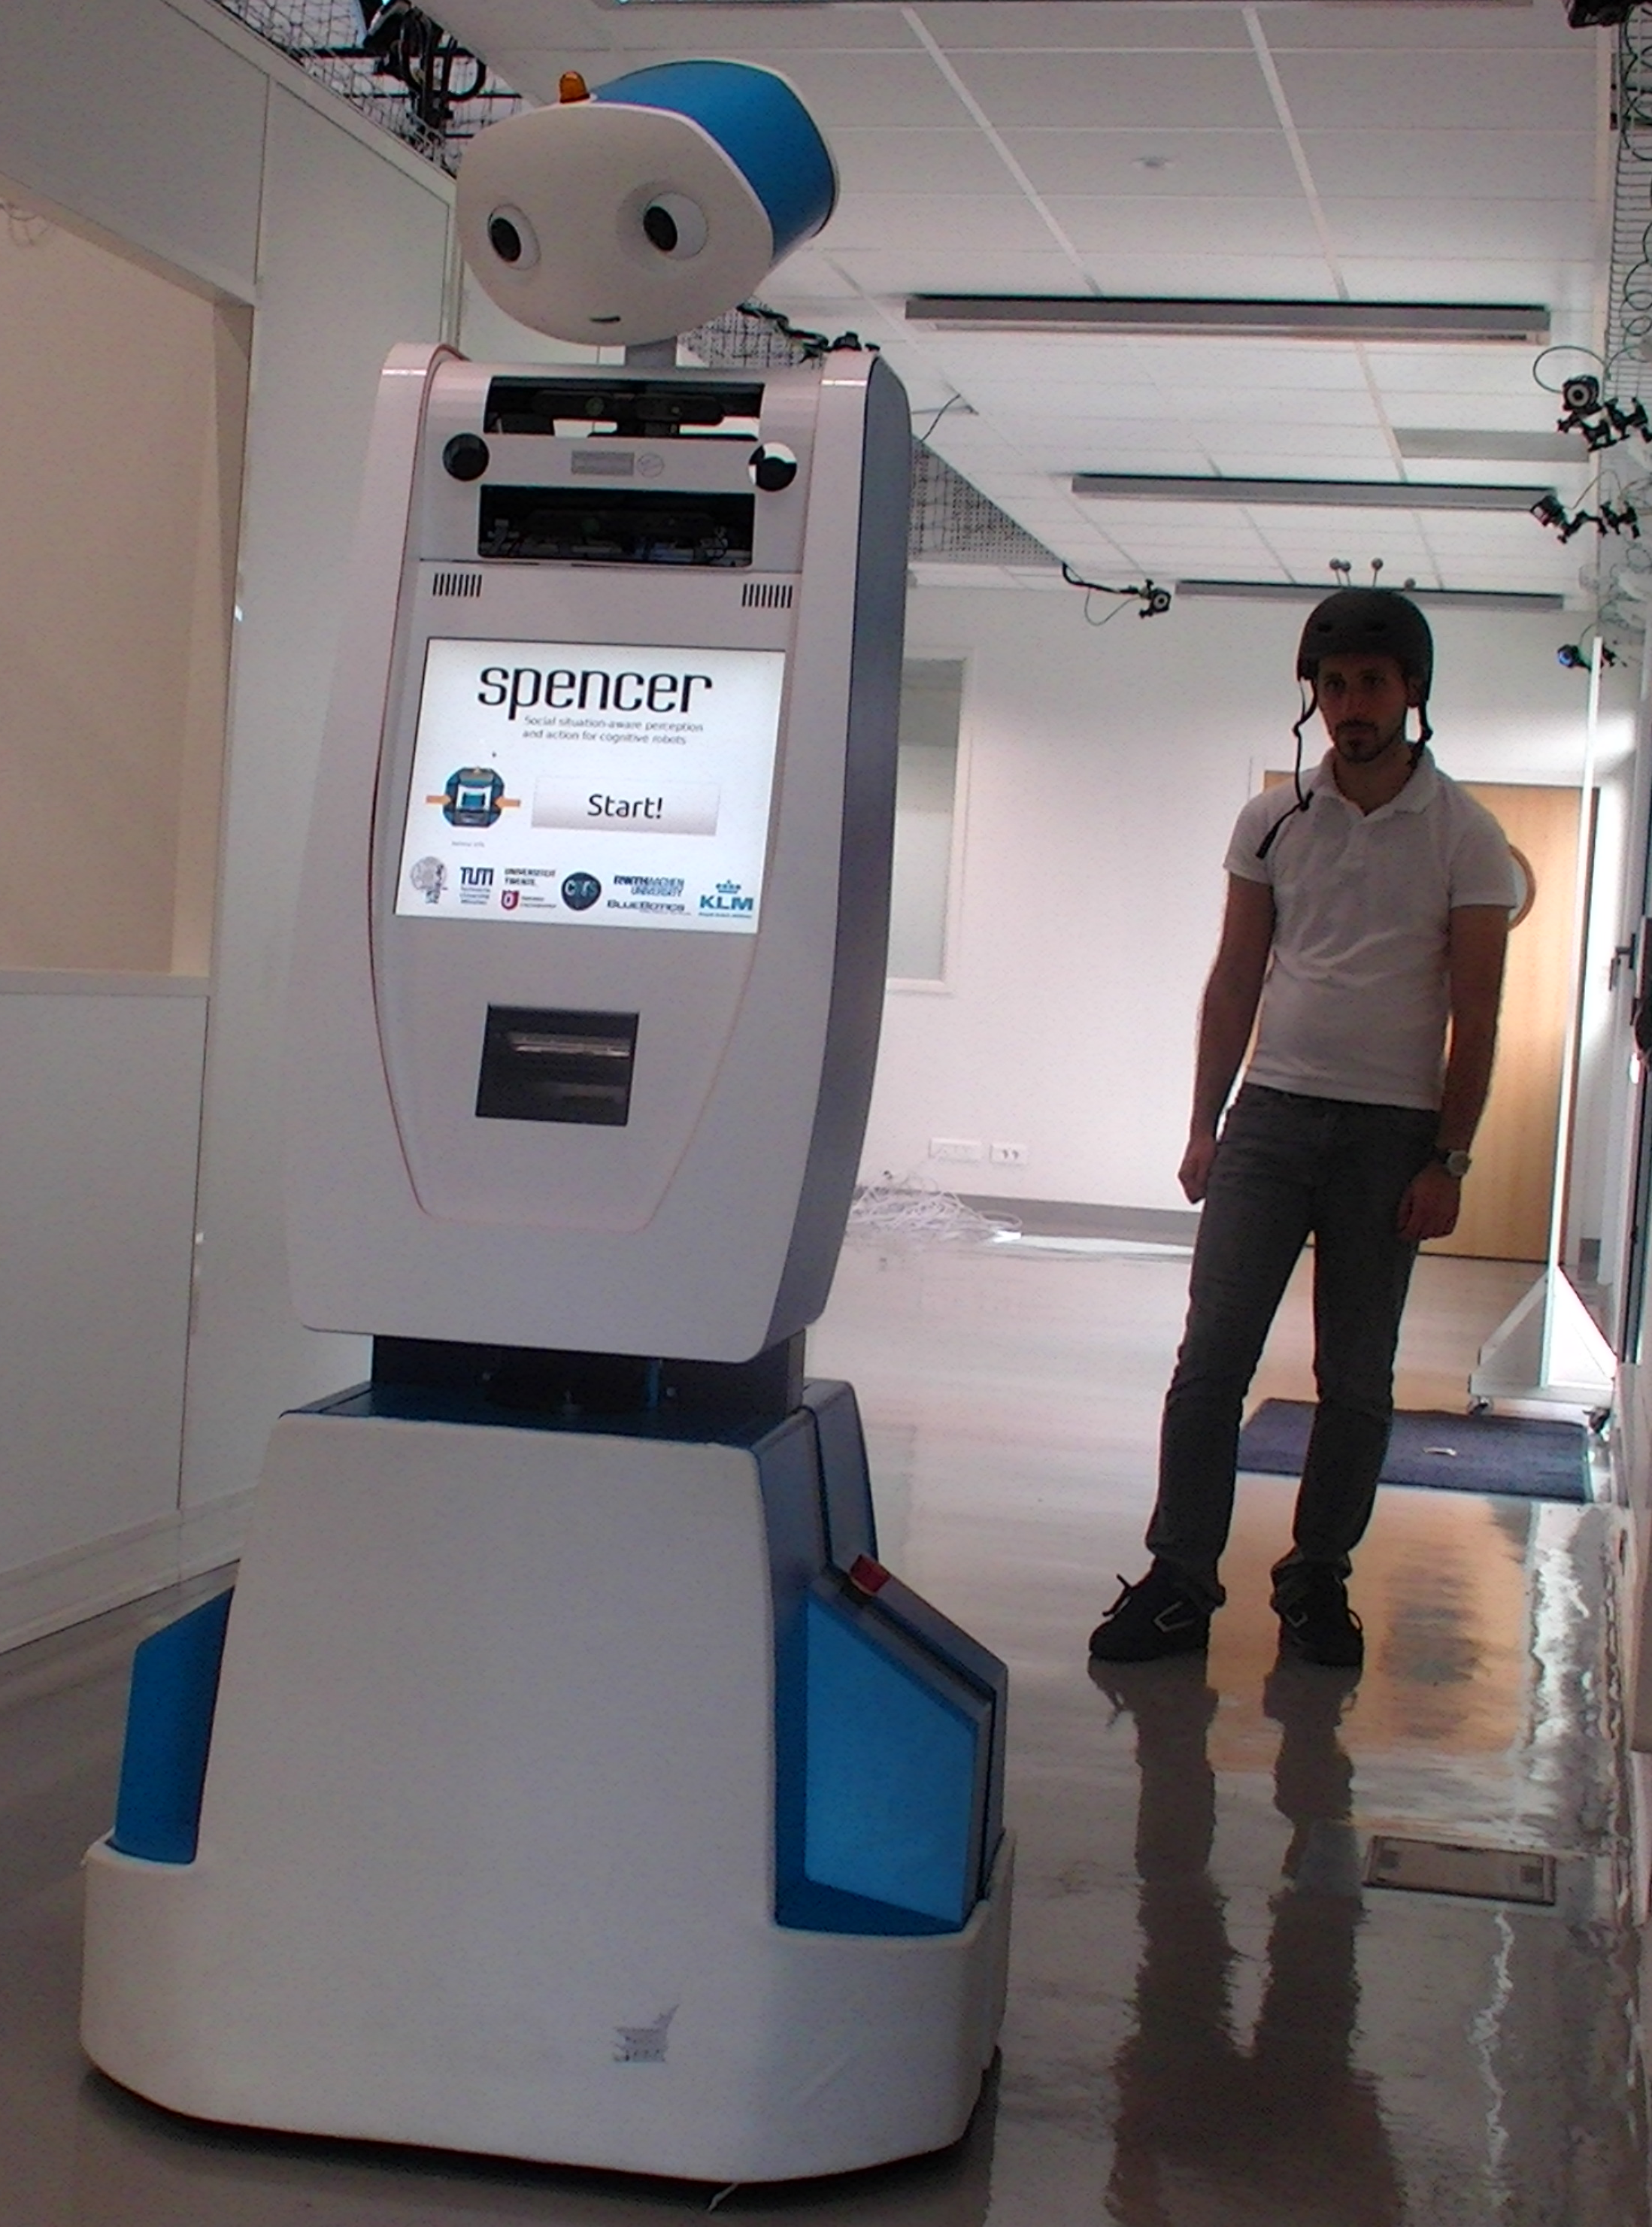
\includegraphics[scale=0.1]{img/robotGuiding.png}
% \caption{second figure}
% \end{minipage}
% \end{figure}

%\lipsum

\begin{table}
 \vspace{-20pt}
\caption{Experiment results: $d$ is the distance between the robot and the user, $s_r$ is the robot's speed, $s_h$ is the human's speed, $\mu$ is the average and $\Delta$ is the variation of the quantity. Distances are expressed in meters, velocities in meters for seconds.}
\centering
\begin{tabular}{ | c | c | c | c | c | }

\hline
  test name     & $\mu$ $distance$ & $\mu$ $speed$ $difference$ & $\Delta$ $distance$ & $\Delta$ $speed$ $difference$ \\
\hline
adapting slow & 2.82 & -0.03 & 0.64 & 0.02 \\
  \hline
  adapting fast & 1.38 & 0.00 & 0.29 & 0.01 \\
  \hline
  no adaptation & 3.08 & -0.09 & 1.04 & 0.07 \\
\hline
proactive slow & 1.45 & -0.06 & 0.04 & 0.10 \\
\hline
proactive fast & 2.66 & -0.11 & 0.63 & 0.01 \\
\hline
\end{tabular}
\label{table:experiment results}
 \vspace{-20pt}
\end{table}


\section{Results on Airport Deployment}


\section{Robot Helper}
\subsection{Experiment Description}
\subsection{Handover}




